\section{AOSP 构建系统}\label{aosp-build-system}

对 AOSP 展开分析的最重要一步是了解 AOSP 的构建过程,而 AOSP 构建系统是解释 AOSP 构建过程的核心关键。本节从 AOSP 构建系统从 GNU Make 到 soong 的演化历史出发,比较了二者在实际应用上的表现并介绍了 soong 中的重要组件与工作方式。

\subsection{AOSP 构建系统历史与现状}

\subsubsection{Android Marshmallow 前:GNU Make}

截至 2015 年上半年,AOSP 所使用的构建系统仍旧依托于 GNU Make——各个模块通过编写各自的 Android.mk 文件,完成对 Android.mk 当前目录下所有源文件的编译以及最终产物的生成。在这一阶段,AOSP 为 GNU Make 提供了统一的编译入口,使用 Makefile 语言的指令将众多仓库下的模块一同构建。由于 GNU Make 的本质是执行给定指令,因此对于使用多种通用编程语言的 AOSP,GNU Make 是一个优秀的顶层构建系统。

然而,随着 AOSP 软件规模的不断增长,GNU Make 逐渐暴露出它的不足之处:

\begin{itemize}
    \item GNU Make 下的 Makefile 文件存在一定的逻辑语句,语法仍较为复杂。Makefile 语法较为灵活,存在诸如分支逻辑、循环逻辑等结构,这为项目开发人员以及软件分析人员带来的较大的困难。
    \item GNU Make 下的 Makefile 需要在每个模块构建之初消除先前模块构建过程中定义的环境变量所带来的影响,进而产生了大量必要且重复的 Makefile 代码。
    \item GNU Make 下的 Makefile 在 AOSP 庞大的系统下,很难在尽量降低对其他模块构建产生影响的同时,对特定模块进行定制化构建工作。
    \item GNU Make 在实际应用过程中,暴露出构建缓慢、难以统一管理等问题。
\end{itemize}

\subsubsection{Android Nought 后:soong / Ninja}

出于对以上问题的考虑,Google 决定将 AOSP Marshmallow 作为最后一个使用 GNU Make 为主要构建系统的大版本,并从 2015 年 1 月起开发适用于 AOSP 的新顶层构建系统——soong。与此同时,Google 采用 Ninja 这一已在 chromium 项目中得到认可的底层构建系统作为代替 GNU Make 构建图生成、构建时资源调度以及提供指令执行环境的工具。

自 Android Nought 开始,AOSP 的构建系统在逐渐从 GNU Make 向 soong / Ninja 过渡。截至目前,AOSP 仍旧存在使用 GNU Make 时期的 Android.mk 文件作为模块构建方式声明的 manifest 文件。

\subsection{soong 的重要组件}

作为 AOSP 的顶层构建系统,soong 需要负责处理 AOSP 内部的复杂性。为了摒除 AOSP 内多语言项目间构建差异与各模块内与模块间引用带来的影响,soong 需要多个组件来完成整体构建过程。

\subsubsection{Blueprint}

在计划逐步抛弃 GNU Make 后,soong 同样需要一种用于描述 AOSP 中各模块内部与模块间的引用关系的文件协议。通过借鉴 Google 公司开发的另一个构建系统 “Bazel.build” 使用的 manifest 语法,soong 对其进行改造后设计形成了以 “bp” 为文件后缀名的 “Blueprint / Android.bp” 文件,用以替换原本各模块中的 Android.mk 文件。 

目前,绝大多数模块使用 Android.bp 文件作为模块构建过程的声明文件(如 framework/base)。对 bp 文件格式的解析需要有一个独立的 Blueprint 模块完成,在当前版本的 soong 中,Blueprint 模块完成了对 bp 文件内容语法语义的解析。

\subsubsection{Kati}

相较于 soong,Kati 为 AOSP 服务的历史更为悠久。在 Android Marshmallow 前,以 GNU Make 为核心的构建体系已经暴露出构建速度不足的缺陷。Kati 起初担负着加速编译的责任。然而随着 soong 的出现与不断完善,AOSP 已经不需要 Kati 加快构建速度。因此 Kati 仅保留了部分功能(即将 Android.mk 文件中内容转化为符合 ninja 文件协议的约定)。

正如上文所述,截至 Android Tiramisu 版本,AOSP 中仍存在部分模块使用 Android.mk 作为模块构建过程的声明文件(如 development/testrunner)。

\subsubsection{Ninja}

Android Nought 后使用已在 chromium 项目中得到认可的 Ninja 作为底层构建工具。

Ninja 将其他构建系统视为 “高级程序设计语言”,同时将自己定位为那些 “高级语言” 对应的 “汇编语言”\cite{NINJABUILD}。也就是说,Ninja 旨在提供一个高效的命令执行环境。任何可用于项目构建的构建系统,都可以将 Ninja 作为构建后端;任何构建系统都可以通过产生内容合乎规范的、以 ninja 为文件后缀的 manifest 文件以借助 Ninja 来加速构建过程。

Ninja 与 GNU Make 类似,不仅是一个构建系统,还定义了用于描述构建过程的文件协议。与 Makefile 相仿,ninja 同样有能力描述有向无环图(DAG)——将文件视作 DAG 中的节点,将输入文件到输出文件的转化过程视作 DAG 中的边。但是,ninja 删除了 Makefile 中的逻辑控制语句,仅仅使用 “输出-输入” 进行描述。

\subsection{soong 的工作流程}

在 soong 运行之初,系统下仅有 soong 系统的源代码,并不能直接使用上述提及的工具。soong 最大的一个特点是允许 “自启动”。在 soong 第一次运行时,系统会自动编译名为 soong\_ui 的二进制文件,该文件作为此后用户使用 soong 其他功能的入口。soong\_ui 的执行也是分阶段的,在初始阶段,soong\_ui 会进行一系列配置,并同时生成名为 Android.bp.list 文件。

此后,soong 进入 minibootstrap 阶段。soong 在本阶段会创建描述构建过程的 manifest 文件并调用 Ninja 开始构建。接下来,soong 进入 bootstrap 阶段,在当前版本 Android Tiramisu 下,soong 并不负责直接构建 AOSP 中的各个模块,而是负责生成 Ninja 所需要的 manifest 文件——build.ninja。因此,与其说 soong 是一个构建系统,不如说 soong 是一个 manifest 文件转换工具。当前版本的 soong 主要由 Blueprint 与 Kati 两个转换工具构成,前者负责使用 soong\_ui 生成的 Android.bp.list 文件收集各模块下的 Android.bp 文件并生成 build.ninja,后者负责收集各模块下仍未调整至 Android.bp 文件的 Android.mk 文件并生成 build-<product>.ninja。最后,soong 会将二者使用 subninja 语法链接到名为 combined-<product>.ninja 文件中,并将该文件输入至 Ninja,作为 Ninja 开展 AOSP 构建过程的输入之一。soong 的整体架构如图 \ref{fig:soong-architecture} 所示。

\begin{figure}
    \centering
    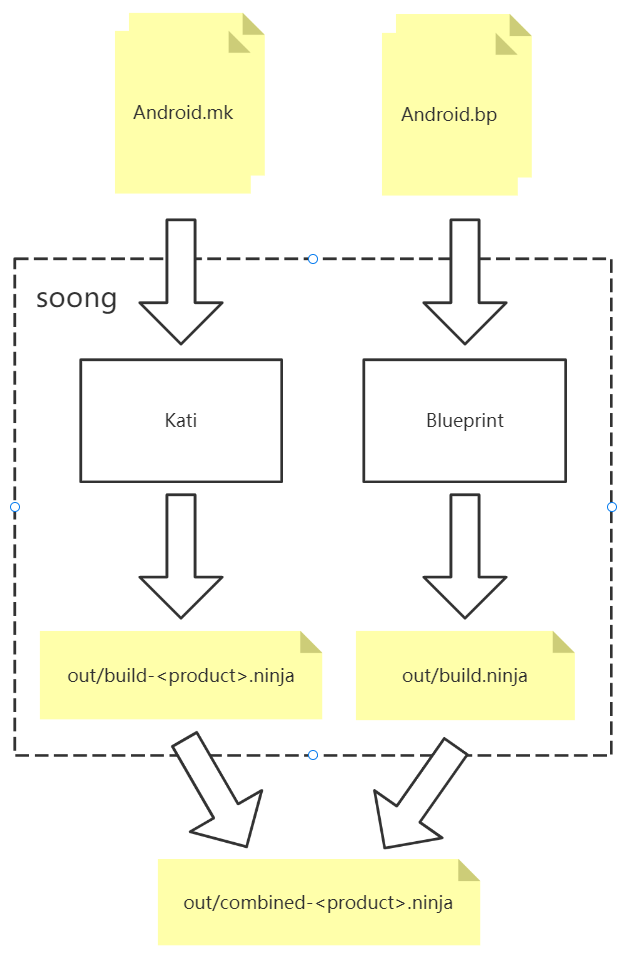
\includegraphics[width=.8\textwidth]{figures/soong-arch.png}
    \caption{soong 构建系统工作示意图}
    \label{fig:soong-architecture}
\end{figure}